\documentclass[a4paper]{article}
\usepackage[T1]{fontenc}			% pacchetto per \chapter
\usepackage[italian]{babel}
\usepackage[italian]{isodate}  		% formato delle date in italiano
\usepackage{graphicx}				% gestione delle immagini
\usepackage{amsfonts}
\usepackage{booktabs}				% tabelle di qualità superiore
\usepackage{amsmath}				% pacchetto matematica
\usepackage{mathtools}				% per sottolineare sotto le equazioni
\usepackage{stmaryrd} 				% per '\llbracket' e '\rrbracket'
\usepackage{amsthm}					% teoremi migliorati
\usepackage{enumitem}				% gestione delle liste
\usepackage{pifont}					% pacchetto con elenchi carini
\usepackage{enumitem}				% pacchetto per elenchi con lettere dell'alfabeto
\usepackage{cancel}					% per cancellare delle espressioni matematiche
\usepackage{listings}				% implementa codice di programmazione


\usepackage[x11names]{xcolor}		% pacchetto colori RGB
% Link ipertestuali per l'indice
\usepackage{xcolor}
\usepackage[linkcolor=black, citecolor=blue, urlcolor=cyan]{hyperref}
\hypersetup{
	colorlinks=true
}

% Colour code style
\definecolor{codegreen}{rgb}{0,0.6,0}
\definecolor{codegray}{rgb}{0.5,0.5,0.5}
\definecolor{codepurple}{rgb}{0.58,0,0.82}
\definecolor{backcolour}{rgb}{0.95,0.95,0.92}

\lstdefinestyle{MATLAB}{
	backgroundcolor=\color{backcolour},   
	commentstyle=\color{codegreen},
	keywordstyle=\color{magenta},
	numberstyle=\tiny\color{codegray},
	stringstyle=\color{codepurple},
	basicstyle=\ttfamily\footnotesize,
	breakatwhitespace=false,         
	breaklines=true,                 
	captionpos=b,                    
	keepspaces=true,                 
	numbers=left,                    
	numbersep=5pt,
	showspaces=false,                
	showstringspaces=false,
	showtabs=false,                  
	tabsize=2
}
\lstset{style=MATLAB}

%\usepackage{showframe}				% visualizzazione bordi
%\usepackage{showkeys}				% visualizzazione etichetta

\newtheorem{theorem}{\textcolor{Red3}{\underline{Teorema}}}
\newtheorem{lemma}{Lemma}
\renewcommand{\qedsymbol}{QED}
\newcommand{\exec}[1]{\llbracket #1\:\rrbracket}
\newcommand{\dquotes}[1]{``#1''}
\newcommand{\longline}{\noindent\rule{\textwidth}{0.4pt}}

\begin{document}
	\author{Università degli Studi di Verona}
	\title{Esame di Elaborazione di segnali e immagini}
	\date{{\Large 01 Febbraio 2021}}
	\maketitle
	
	\section{Esercizio (10 punti)}
	
	Sia $g\left(t\right)$ un segnale di durata indefinita la cui funzione nel tempo è definita come:
	\begin{equation*}
		g\left(t\right) = 40\mathrm{sinc}\left(20t\right) + 15\mathrm{sinc}\left(30t\right) e^{-j 2 \pi 45 t} + 15\mathrm{sinc}\left(30t\right) e^{j 2 \pi 45 t}
	\end{equation*}
	Descrivere analiticamente e graficamente, in frequenza, il segnale $G\left(\mu\right)$.\newline
	
	\noindent
	Si descriva inoltre:
	\begin{itemize}
		\item Analiticamente, in frequenza e nel tempo
		\item Graficamente, in frequenza
	\end{itemize}
	Le elaborazioni a cui il segnale $g\left(t\right)$ è sottoposto se ad esso vengono applicate in sequenza le operazioni schematizzate nel sistema sottostante.
	\begin{figure}[!htp]
		\centering
		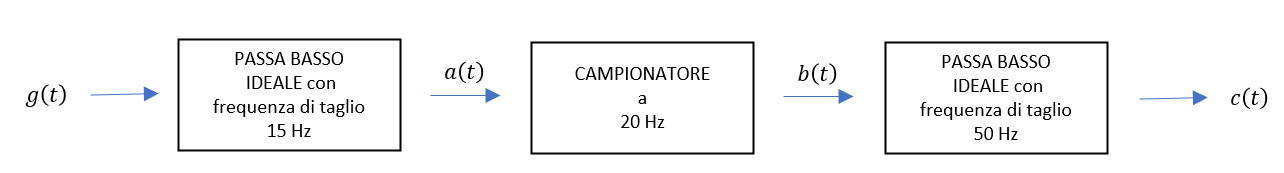
\includegraphics[width=\textwidth]{img/fig_1.png}
	\end{figure}
	
	\section{Esercizio (9 punti)}
	
	Valutare graficamente il prodotto di convoluzione $y\left(t\right) = x\left(t\right) * h\left(t\right)$.
	\begin{figure}[!htp]
		\centering
		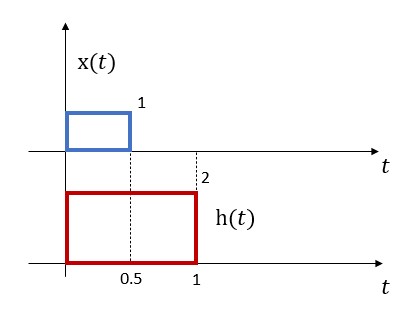
\includegraphics[width=.51\textwidth]{img/fig_2.png}
	\end{figure}\newpage

	\section{Esercizio (6 punti)}
	
	\begin{enumerate}[label=\alph*)]
		\item Cosa si intende per filtro passa basso \dquotes{ideale}? Quali sono gli effetti del suo utilizzo nel dominio duale?
		
		\item Quanti e quali tipi di rumore associato alle immagini abbiamo visto a lezione? Se ne dettagli almeno uno in maniera approfondita, unitamente al filtraggio che lo elimina/attutisce in maniera più efficace.
		
		\item Con che misura si descrive il rumore? Darne una definizione analitica.
	\end{enumerate}
\end{document}